\section*{Figures}

\listoffigures

\clearpage

\begin{figure}[tbhp!] \centering
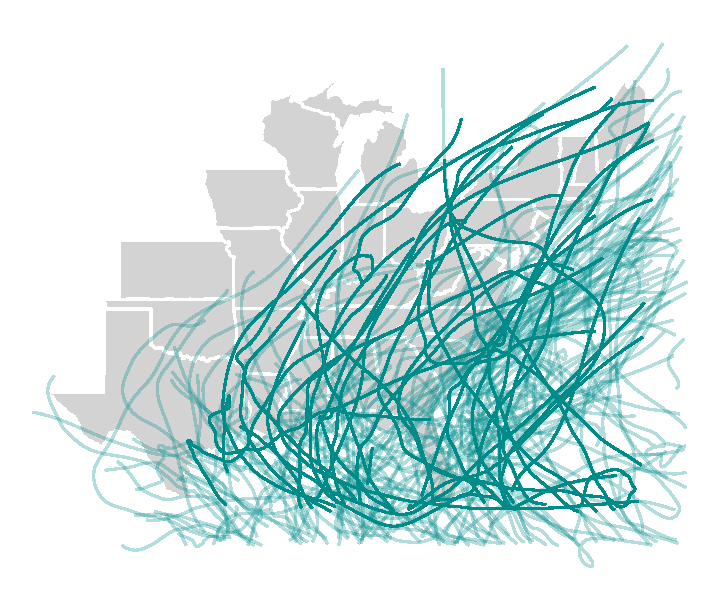
\includegraphics[width=\linewidth]{hurrtracks}
\caption{Study area and storms considered in this study. All counties in the states
	shown in this map were investigated. The lines show the paths of the
	study storms, which included all tracked storms in 1988\,--\,2018 that
	are recorded in \ac{HURDAT2} and that came
	within 250~\si{\kilo\metre} of at least one \ac{US} county. Thicker
	lines show the tracks of storms whose names have been retired,
	indicating that the storm was particularly severe or had notable
	impacts.  }
\label{fig:hurrtracks}
\end{figure}

\clearpage

\begin{figure}[tbhp!] \centering
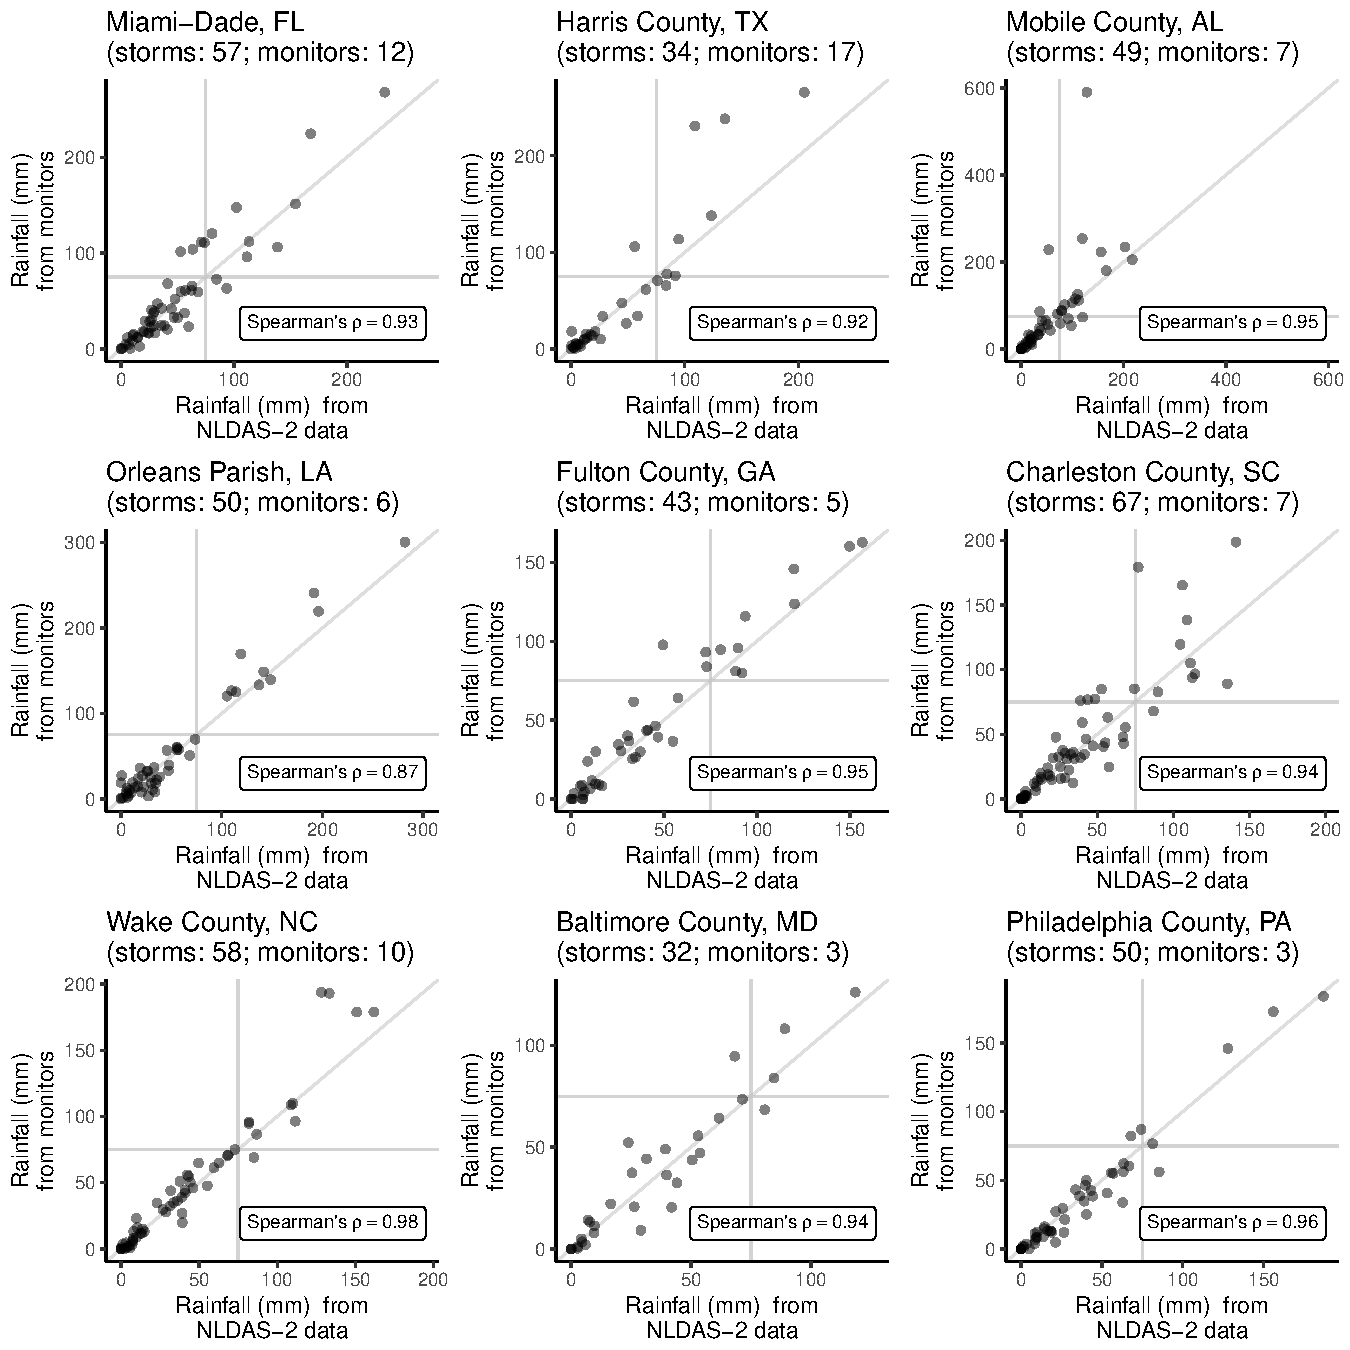
\includegraphics[width=\linewidth]{raincomparison} 
	\caption{Comparison in nine sample counties of two sources of storm-associated 
	rainfall estimates: (1) county-level estimates derived from 
	a re-analysis dataset and (2) county-level estimates based on ground-based
	observations in nine sample counties. For both, estimates  
	include rainfall from two days before to one day after the storm's closest
	approach to the county. Each small graph shows data for one sample county, 
	and each point shows one tropical storm. The number of storms 
	within each county and the number of ground-based monitors reporting precipitation during 
	the county's storms are given above each plot. Horizontal and vertical lines 
	in each plot show the threshold of 75~\si{\milli\metre} used to classify a storm 
	as ``exposed'' for the binary classification considered for this metric 
	in further analysis (Table 1). Note that 
	ranges of the x- and y-axes differ across counties.
	} 
\label{fig:raincomparison}
\end{figure}

\begin{figure}[tbhp!]
\centering
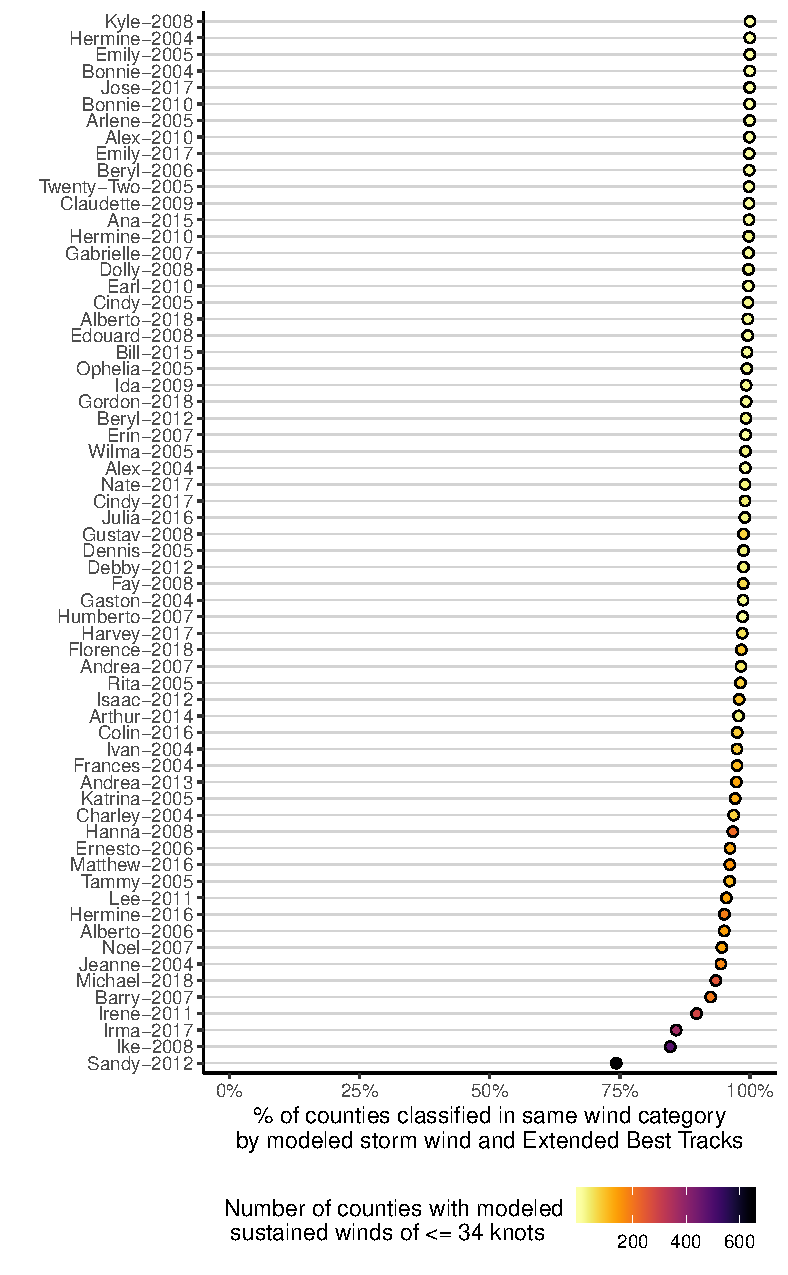
\includegraphics[width=0.8\linewidth]{windcomparison}
	\caption{Comparison of two sources of wind exposure estimates: 
	(1) modeled peak sustained surface wind 
	and (2) estimates based on \ac{HURDAT2}'s wind speed radii.
	Each point represents a storm, with the x-axis giving the percent of
	counties classified in the same category of peak sustained surface
	wind ($<$34~kt; 34\,--\,49.9~kt;
	50\,--\,63.9~kt; $\ge$64~kt) by both sources of 
	data. The color of each point gives the number of study counties that were exposed to
	peak sustained surface wind of at least 34~kt (based
	on modeled wind). Estimates are shown for study storms since
	2004, the earliest year for which post-storm reanalysis wind speed
	radii are routinely available in \ac{HURDAT2}, and for which at
	least one study county had a peak sustained wind of $\ge$34~\si{\knot}
	based on the post-storm wind radii.
	}
\label{fig:windcomparison}
\end{figure}

\begin{figure}[tbhp!]
\centering
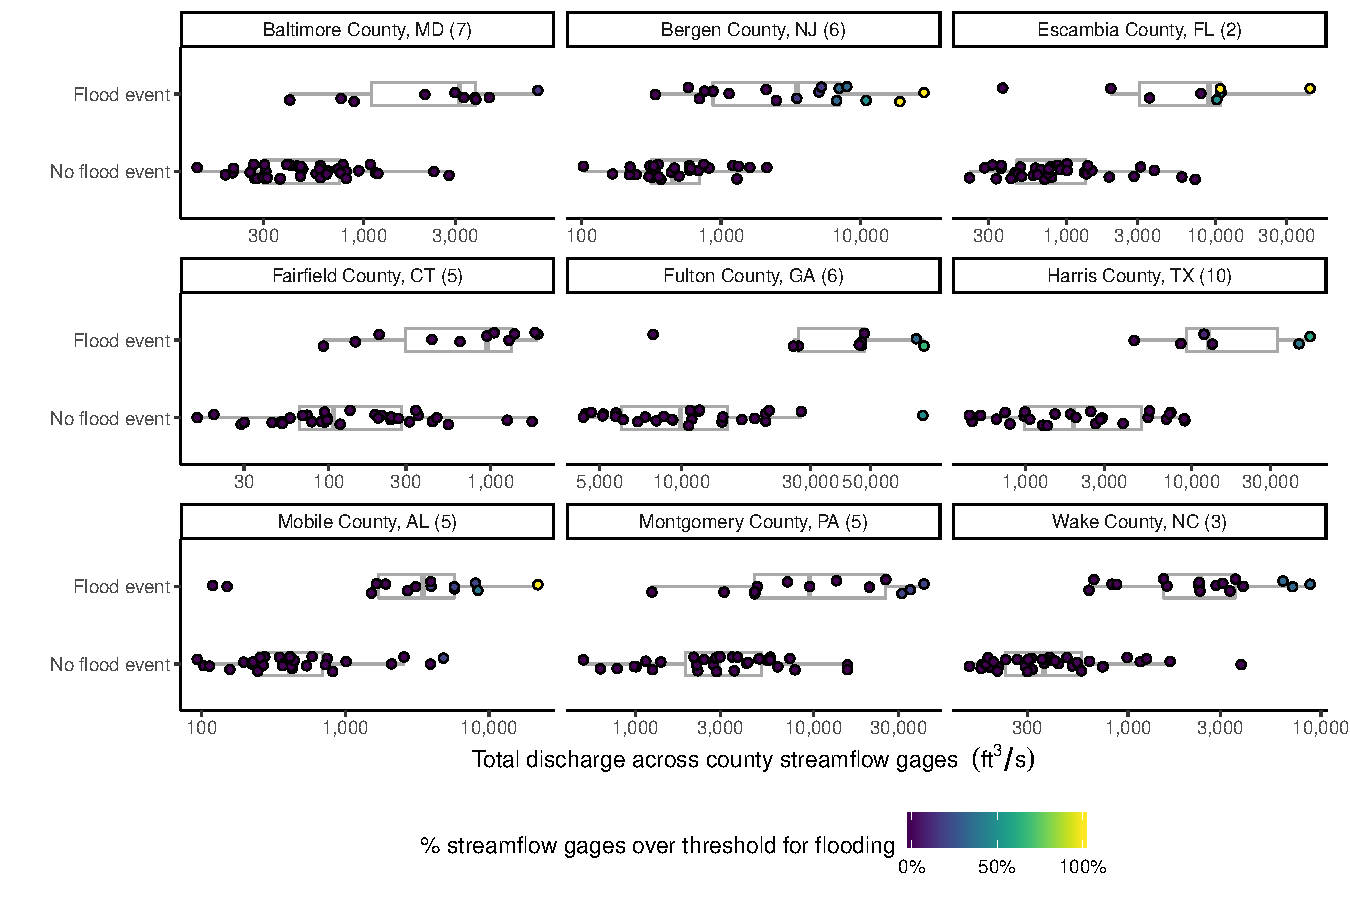
\includegraphics[width=\linewidth]{floodcomparison}
\caption{Comparison in nine sample study counties of flood status based on
	two data sources: (1) NOAA Storm Events listings matched to \ac{HURDAT2} storm track data
	and (2) county streamflow gages. Each small plot shows results for one of the sample
	counties. Each point represents a single tropical storm, and the
	point's position along the x-axis shows the highest daily total
	streamflow (cubic feet per second) during the five-day window surrounding the storm, 
	summed across all identified
	streamgages in the county. The y-axis separates storms
	for which a flood event was reported in NOAA's Storm Events database
	in the county with a start date within the five-day window of the
	storm's closest approach. The color of each point gives
	the percent of streamflow gages in the county with a daily streamflow
	that exceeded a threshold of flooding (the streamgage's median value
	for annual peak flow) on any day during the five-day window. The number
	of streamflow gages used in analysis are given in parentheses beside
	the county's name in the panel title.  Note that the x-axis scales
	differ by county, depending on the number of streamflow gages and
	typical flow rates for each gage, and are on a log-10 scale.
	}
\label{fig:floodcomparison}
\end{figure}

\clearpage

\begin{figure}%[tbhp] 
\centering
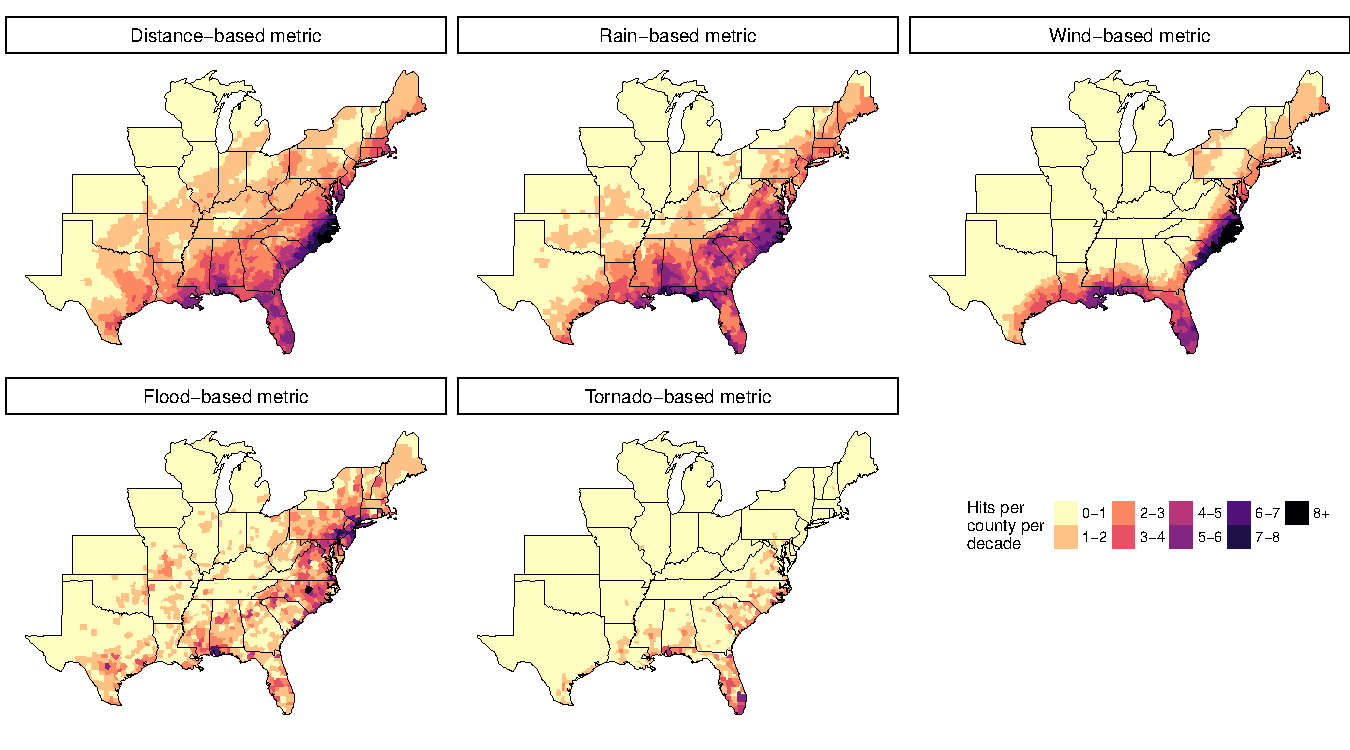
\includegraphics[width=7cm]{averageexposureonly.pdf} 
\caption{Average number of county-level storm exposures per decade for binary 
	classifications based on each
	single-hazard exposure metric (Table \ref{tab:exposuremetrics}). The years used to
	estimate these averages are based on years of available exposure data
	(rain: 1988\,--\,2011; wind:~1988\,--\,2018; flood events:~1996\,--\,2018; and
	tornado events:~1988\,--\,2018). } 
\label{fig:averageexposure} 
\end{figure}

\clearpage

\begin{figure}%[tbhp]
\centering
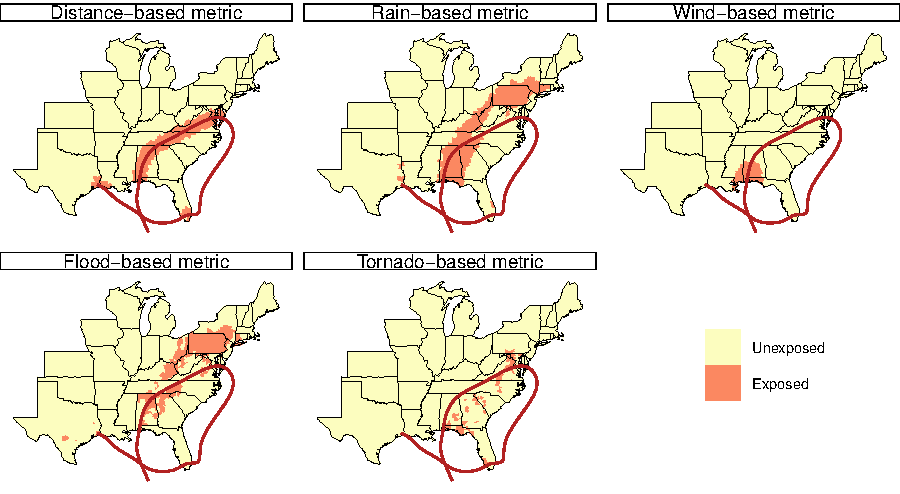
\includegraphics[width=\textwidth]{ivanonly.pdf}
\caption{Counties classified as exposed to Hurricane Ivan in 2004 under each
	exposure metric considered (Table~\ref{tab:exposuremetrics}). The red
	line shows the track of Hurricane Ivan based on
	\ac{HURDAT2}.  Similar maps for other
	large-extent storms are given in Figure~S4.
	}
\label{fig:ivanexposure} 
\end{figure}

\clearpage

\begin{figure}%[tbhp] 
	\centering 
	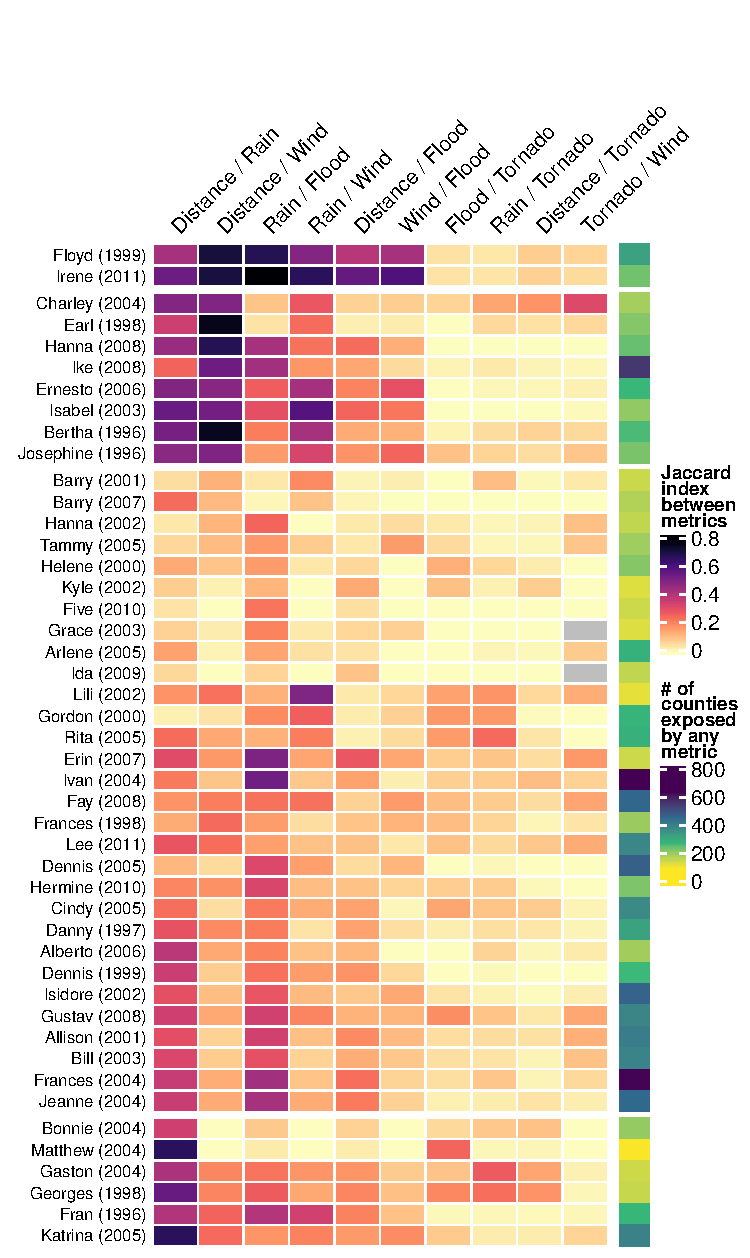
\includegraphics[width = 0.8\linewidth]{jaccard_heatmap.pdf}
	\caption{Agreement between exposure classifications based on different
	single-hazard exposure metrics for all storms between~1996 and~2011 for
	which at least~100 counties were exposed based on at least one metric.
	Each row shows one storm, and the color of each cell shows the measured
	Jaccard index for each pair of exposure metrics (proportion of counties
	classified as exposed by both metrics out of counties classified as
	exposed by either metric). For Grace in 2003 and Ida in 2009, there
	were no county exposures for either the tornado-based metric or the
	wind-based metric (indicated by gray squares). Colors to the right of
	the heatmap show the number of exposed counties based on any of the
	metrics, and this panel is linked with the color scale labeled ``\# of
	counties exposed by any metric''. Storms are displayed within clusters
	that have similar patterns based on hierarchical clustering.}
\label{fig:jaccard} 
\end{figure}


\begin{comment}
\clearpage

\begin{figure*}%[tbhp]
\centering
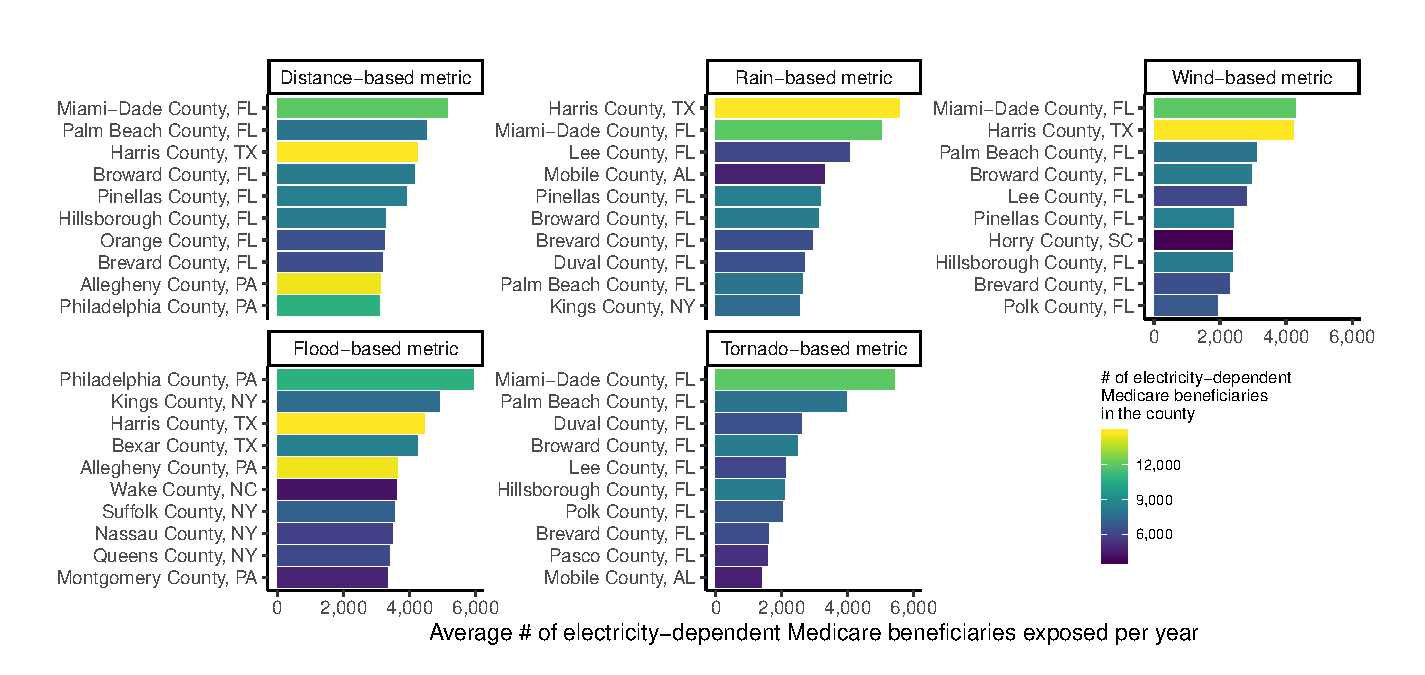
\includegraphics[width=15.5cm]{topelecdependexposure}
\caption{Study counties with the highest expected rate of physical exposure per year among
	 electricity-dependent Medicare beneficiaries based on each exposure metric. 
	 The color of each bar indicates the number of Medicare beneficiaries in the 
	 county reliant on electricity-dependent medical and assistive equipment as 
	 of July~2017. The length of each bar shows the average expected rate of physical exposure
	 to tropical cyclones among this population based on a given exposure metric, i.e., 
	 the expected number of these electricity-dependent Medicare beneficiaries exposed 
	 to tropical storms per year based on that metric (Table 1).}
\label{fig:topelecdependexposure}
\end{figure*}

\end{comment}
